157. \begin{figure}[ht!]
\center{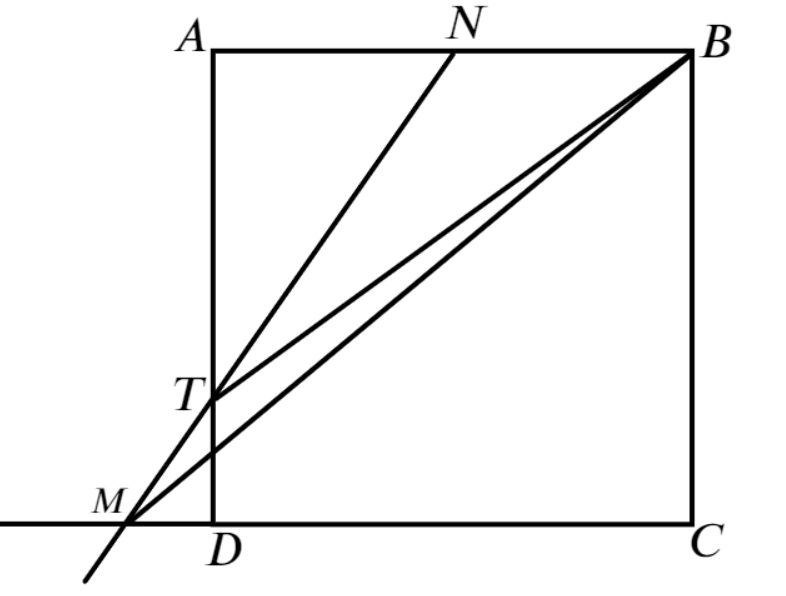
\includegraphics[scale=0.35]{g9-157.png}}
\end{figure}\\
$tg(\angle TNA)=\cfrac{TA}{NA}=0,5,$ значит $TA=0,5\cdot4=2.$ Тогда $S_{\Delta BMT}=S_{\Delta BMN}-S_{\Delta BTN}=\cfrac{1}{2}\cdot8\cdot4-\cfrac{1}{2}\cdot2\cdot4=12$ (площади посчитаны через высоты, опущенные из точек $M$ и $T$).\newpage\noindent
